\section{PPU}
\label{sec:tp-ppu}

Obrazový procesor (PPU -- \textit{Picture Processing Unit}) je hlavní komponentem systému NES
zodpovědným za generování výsledného video signálu na základě dat z procesoru a grafických dat
uložených na herní kazetě. PPU generuje kompozitní signál sestávající z 262 řádků
(\textit{scanlines}), z nichž je 240 viditelných.

PPU funguje na principu dlaždicové grafiky, kde pozadí je rozděleno na menší bloky (dlaždice) o
velikosti 8\texttimes8 pixelů. Samotné dlaždice se uchovávají v CHR pamětí kazety, která je mapována
do adresního prostoru PPU. Také PPU je vybaven 8 paletami.

\subsection{Paměťová organizace a sběrnice}

PPU disponuje vlastní sběrnicí, ke které je připojena interní video paměť (VRAM) a dlaždicová paměť
na kazetě (CHR) (tabulka \ref{tab:ppu_map}). Pro potřeby emulace je zásadní rozlišovat mezi
vykreslováním pozadí a pohyblivých objektů (spritů), neboť každý z těchto prvků využívá jinou část
paměťové hierarchie.

\begin{table}
    \centering
    \begin{tabular}{llp{5cm}l}
        \toprule
        \textbf{Adresní rozsah} & \textbf{Velikost} & \textbf{Účel} & \textbf{Mapování} \\
        \midrule
        \texttt{\$0000}--\texttt{\$0FFF} & 4096 B & Tabulka vzorů 0 (Pattern Table) & Kazeta \\
        \texttt{\$1000}--\texttt{\$1FFF} & 4096 B & Tabulka vzorů 1 (Pattern Table) & Kazeta \\
        \texttt{\$2000}--\texttt{\$23BF} & 960 B  & Jmenná tabulka 0 (Nametable)   & Interní/VRAM \\
        \texttt{\$23C0}--\texttt{\$23FF} & 64 B   & Tabulka atributů 0             & Interní/VRAM \\
        \texttt{\$2400}--\texttt{\$2FFF} & ---    & Zrcadlení jmenných tabulek 1-3 & Dle zapojení \\
        \texttt{\$3F00}--\texttt{\$3F0F} & 16 B   & Paleta pozadí                  & Interní \\
        \texttt{\$3F10}--\texttt{\$3F1F} & 16 B   & Paleta spritů                  & Interní \\
        \bottomrule
    \end{tabular}
    \caption{Paměťová mapa PPU.}
    \label{tab:ppu_map}
\end{table}

Fyzicky PPU obsahuje pouze 2 KiB paměti pro jmenné tabulky (dostačující pro dvě tabulky), zbývající
dvě logické tabulky jsou řešeny zrcadlením (\textit{mirroring}), které může být horizontální nebo
vertikální v závislosti na hardwarovém zapojení na kazetě (mapperu).

\subsection{Vystavené registry}

PPU mapuje devět registrů do adresního prostoru CPU:

\begin{enumerate}
    \item \texttt{PPUCTRL} - základní nastavení činnosti PPU
    \item \texttt{PPUMASK} - nastavení procesu vykreslování
    \item \texttt{PPUSTATUS} - stavový registr (V-Blank, NMI; jenom pro čtení)
    \item \texttt{PPUSCROLL} - nastavení scrollingu
    \item \texttt{PPUADDR} - adresa do VRAM
    \item \texttt{PPUDATA} - data do VRAM
    \item \texttt{OAMADDR} - adresa do primárního OAM
    \item \texttt{OAMDATA} - data do primárního OAM
    \item \texttt{OAMDMA} - DMA kanál do primárního OAM
\end{enumerate}

\subsection{Vzory dlaždic a tabulky vzorů (Pattern Tables)}

Vzory dlaždic jsou uloženy v tabulkách vzorů v paměti CHR na kazetě. Aby se ušetřilo místo, NES
využívá metodu bitových rovin (\textit{bitplanes}). Každý řádek dlaždice je definován dvěma byty:
první byte obsahuje nižší bity barvy pro 8 pixelů, druhý byte (uložený o 8 bytů dále) obsahuje vyšší
bity. Výsledkem je 2bitový index (hodnota 0--3), který určuje barvu pixelu v rámci zvolené palety
(obr. \ref{fig:sprite_bitplanes}).

PPU je schopen adresovat pouze 2 tabulky vzorů. Existují však mappery, které implementují
přepínání banek tabulek vzorů a proto dovolují používat více než 2 tabulky.

\begin{figure}[H]
    \centering
    \begin{subfigure}{0.45\textwidth}
        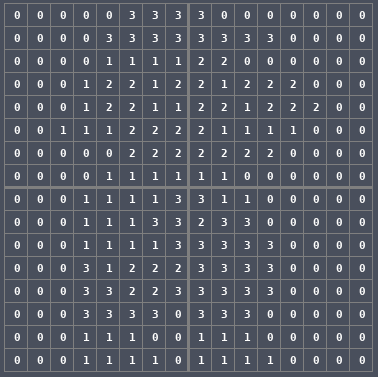
\includegraphics[height=6cm]{images/sprite_02.png}
        \caption{Rozvržení spritu s indexy do palety (barva 0 je průhledná).}
        \label{fig:sprite_colorless}
    \end{subfigure}
    \quad
    \begin{subfigure}{0.45\textwidth}
        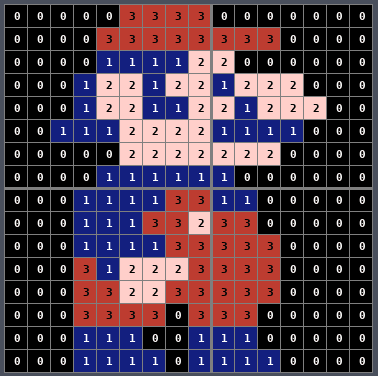
\includegraphics[height=6cm]{images/sprite_03.png}
        \caption{Obarvený sprite (barvy závisejí na specifikované paletě v metadatech spritu).}
        \label{fig:sprite_colorful}
    \end{subfigure}
    \caption{Indexování do palet pomocí bitových rovin. Zdroj \cite{austinmorlan-nes}.}
    \label{fig:sprite_bitplanes}
\end{figure}

\subsection{Jmenné tabulky (Nametables)}

Jmenná tabulka definuje rozvržení pozadí obrazovky. Skládá se z 30 řádků po 32 dlaždicích, přičemž
každý byte v tabulce představuje index dlaždice z \textit{Pattern Table}.

% Jednou z nejpokročilejších
% funkcí PPU ve své době byl hardwarový scrolling na úrovni jednotlivých pixelů. Tento mechanismus
% umožňuje definovat výřez (\textit{viewport}) do většího pozadí tvořeného jmennými tabulkami, což
% umožňuje plynulý pohyb scény bez nutnosti překreslovat celou paměť.

\subsection{Tabulky atributů (Attribute Tables) a palety}

Vzhledem k limitacím hardwaru nemůže mít každá dlaždice vlastní libovolnou barvu. Tabulka atributů
(posledních 64 bajtů v každé jmenné tabulce) rozděluje obrazovku na bloky 4\texttimes4 dlaždice
(tzv. metatily). Každý bajt v této tabulce určuje paletu pro čtyři sousedící skupiny dlaždic (každá
o velikosti 2\texttimes2 dlaždice).

\begin{figure}[H]
    \centering
    
\includegraphics[width=0.5\textwidth]{images/palette.png}
    \caption{Hardwarová paleta systému NES. Zdroj \cite{nes-palette}.}
    \label{fig:nes-palette}
\end{figure}

PPU využívá celkem 8 palet po 4 barvách (4 pro pozadí a 4 pro sprity). První barva v každé paletě je
považována za průhlednou (u pozadí se místo ní vykresluje barva pozadí z paměti \texttt{\$3F00}).
Ačkoliv PPU interně pracuje s 53 barvami (obr. \ref{fig:nes-palette}), díky speciálním bitům v
registru \texttt{PPUMASK} a přesnému časování (tzv. \textit{color emphasis}) lze dosáhnout širší
barevné škály.\cite{nes-palettes-tricks}

\subsection{Objekty a sprity (OAM)}

Data o spritech jsou uložena ve vyhrazené paměti \textbf{primární OAM}
(\textit{Object Attribute Memory}) o velikosti 256 bytů, což umožňuje definovat až 64 spritů. Každý
sprite se skládá z 4 bytů: souřadnice Y, index dlaždice, atributy (horizontální a vertikální
zrcadlení, index palety, priorita vůči pozadí) a souřadnice X.

\subsection{Evaluace spritů (prohledávání OAM)}
\label{tp:sprite-eval}

Jednou za scanline, PPU nezávisle na vykreslování prohledává primární OAM paměť pro vykreslení
dalších řádků spritů. Vybírá nejvýše 8 spritů a kopíruje jejích data do vnitřní mezipaměti
(\textit{sekundární OAM}), které pak využije k vykreslení řádků spritů.

\subsection{Sprite overflow}

V případě, pokud při prohledávání primární OAM již se zaplnil sekundární OAM, PPU ukončí tento
proces a nastaví příznak \textbf{sprite overflow}. Z důvodu chyby v původním návrhu hardwaru NES,
logika detekce přetečení spritů nebyla správná, proto tento příznak se téměř nepoužívá.

\subsection{Scrolling}

Jednou z klíčových vlastností grafického procesoru PPU je podpora scrollování (plynulého posunu)
pozadí na úrovni jednotlivých pixelů, a to v horizontálním i vertikálním směru. Tento mechanismus
umožňuje definovat výřez (\textit{viewport}) do paměťového prostoru pozadí, který je větší než
samotná viditelná plocha obrazovky. Díky tomu nejsou hry omezeny na jedinou statickou scénu, ale
mohou vytvářet rozsáhlé herní světy přesahující rozlišení monitoru.

\begin{figure}[H]
    \centering
    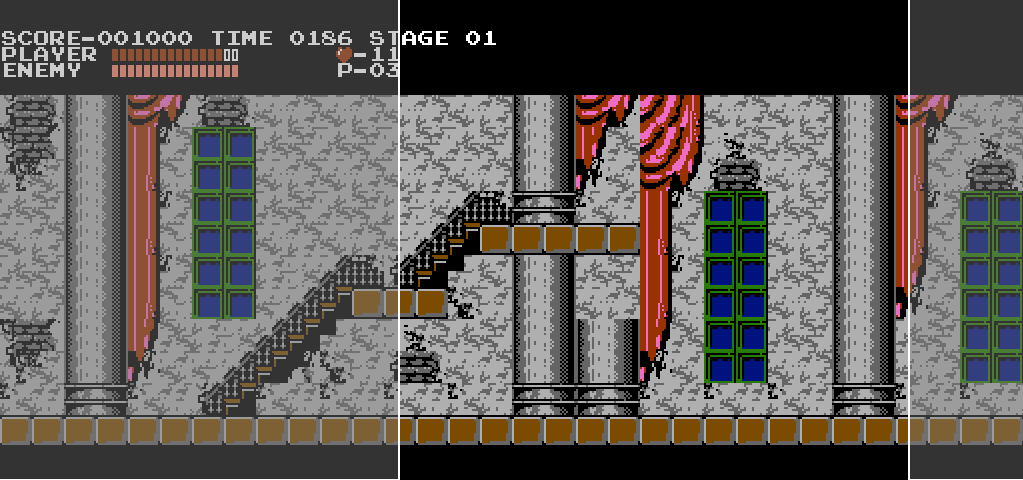
\includegraphics[width=0.75\textwidth]{images/scrolling.png}
    \caption{Znázornění scrollingu: šedé obdélníky vyznačují viditelnou část jmenných tabulek,
    zatímco oblast mezi nimi není hráčem viditelná. Hry předem zapisují do neviditelných
    oblastí jmenných tabulek další dlaždice mapy. Je zde také patrné zrcadlení jmenných tabulek.
    Pořízeno z emulátoru Mesen.}
    \label{fig:scrolling}
\end{figure}

Ačkoliv každá jmenná tabulka popisuje fixní mřížku dlaždic (32×30), scrollování není omezeno
hranicemi jedné konkrétní tabulky. Zásadní roli zde hraje zrcadlení, které definuje mapování
fyzických jmenných tabulek v adresním prostoru paměti VRAM. V okamžiku, kdy výřez obrazu překročí
hranici aktuální tabulky, zrcadlení určuje, která data budou interpretována jako navazující.
Zrcadlení tak efektivně určuje preferovaný směr (horizontální či vertikální), ve kterém může
probíhat plynulý posun obrazu bez vzniku grafických artefaktů (obr. \ref{fig:scrolling}).

Pozice výřezu je definována kombinací souřadnic dlaždic a jemných pixelových offsetů v registrech
\texttt{PPUSCROLL} a \texttt{PPUADDR}.

\label{tp:ppu-loopy}
Přesná hardwarová implementace scrollování v původním čipu PPU nebyla po dlouhou dobu veřejně známa.
V komunitě vývojářů emulátorů se však stal standardem tzv. \textbf{Loopyho model}\footnote{Autorem
je uživatel fóra NESDev s přezdívkou ,,Loopy'', který model odvodil na základě reverzního inženýrství
a pozorování reálného hardwaru.}. Tento model popisuje vnitřní registry PPU a jejich specifické
chování během vykreslovacího cyklu, což umožňuje dosáhnout vysoké věrnosti emulace i u technicky
náročných her (zápis do registrů scrollu během vykreslování, diagonální směr scrollingu apod.).

\subsection{Proces vykreslování a časování}

Vykreslování probíhá cyklus po cyklu v rámci každého řádku. Z hlediska emulace je důležité rozlišení
fází:

\begin{enumerate}
    \item \textbf{Pre-render scanline (-1 nebo 261):} PPU se připravuje na snímek, plní vnitřní registry a
        čistí příznaky V-Blank a Sprite 0 Hit.
    \item \textbf{Visible scanlines (0--239):} Probíhá samotné generování obrazu. V této fázi PPU
        neustále přistupuje k paměti, proto by CPU nemělo do VRAM zapisovat (hrozí grafické
        artefakty, ačkoliv velké množství programů to ignoruje).
    \item \textbf{Post-render scanline (240):} Neaktivní řádek.
    \item \textbf{V-Blank (241--260):} Obraz se nevykresluje. Na začátku této fáze se nastaví příznak
        \mbox{V-Blank} a generuje se přerušení NMI. Toto je bezpečné okno pro CPU k aktualizaci
        grafických dat a přenosu dat do OAM.
\end{enumerate}
